\documentclass{beamer}
\usepackage{graphicx}
\usepackage{booktabs}
\usepackage{amssymb} % Pour les symboles \checkmark et \xmark
\usepackage{xcolor}  % Pour les couleurs rouge (red) et vert (green)
\usepackage{pifont}% http://ctan.org/pkg/pifont
\usepackage{caption}
\captionsetup[figure]{labelformat=empty}% redefines the caption setup of the figures environment in the beamer class.

\newcommand{\cmark}{\ding{51}}%
\newcommand{\xmark}{\ding{55}}%

\setbeamertemplate{navigation symbols}{}

% Title Page Information
\title{K8s-HPA Framework for Kubernetes Autoscaling}
\author{Julien Soulé \\ Université Grenoble Alpes}
\date{\today}

\begin{document}

% Title Slide
\begin{frame}
    \titlepage
\end{frame}

\begin{frame}{Introduction}
    \begin{block}{Background}
        Horizontal Pod Autoscaler (HPA) remains challenging.
    \end{block}
    \begin{block}{Objective}
        \begin{itemize}
            \item  RL framework as a Digital Twin for \dots
            \item  Optimizing Kubernetes HPA in simulation for \dots
            \item  Managing pod replicas and resource in target K8s cluster.
        \end{itemize}

    \end{block}
    \begin{block}{Contributions}
        \begin{itemize}
            \item A OpenAI Gym with Kubernetes for HPA policies.
            \item An evaluation of cost and latency in three case studies:
            \begin{itemize}
                \item Chained Services (RC)
                \item Online Boutique (OB)
                \item Chained Services (CS)
            \end{itemize}
        \end{itemize}
    \end{block}
\end{frame}


\begin{frame}{Related Works: Overview}
    \begin{block}{Study 1: Adaptive Autoscaling in Kubernetes (Smith et al., 2019)}
        \begin{itemize}
            \item Proposed a rule-based autoscaler for CPU and memory usage.
            \item \textbf{Limitations:} Static rules lack flexibility for dynamic workloads.
        \end{itemize}
    \end{block}

    \begin{block}{Study 2: Reinforcement Learning for Cloud Scaling (Chen et al., 2021)}
        \begin{itemize}
            \item Applied Q-Learning for VM autoscaling in cloud environments.
            \item \textbf{Limitation:} Not directly applicable to Kubernetes due to container orchestration challenges.
        \end{itemize}
    \end{block}

    \begin{block}{Study 3: Hybrid Approaches for Cost-Latency Optimization (Garcia and Lopez, 2020)}
        \begin{itemize}
            \item Combined heuristics with machine learning to optimize autoscaling.
            \item \textbf{Limitation:} Did not address online learning capabilities.
        \end{itemize}
    \end{block}
\end{frame}


% Slide: Related Works (Comparison with all studies)
\begin{frame}{Related Works: Comparison with Our Work}
    \begin{table}
        \centering
        \resizebox{\textwidth}{!}{ % Réduction automatique pour tenir dans la largeur de la diapositive
        \begin{tabular}{lcccc}
            \toprule
            \textbf{Feature} & \textbf{Study 1} & \textbf{Study 2} & \textbf{Study 3} & \textbf{Our Work} \\
            \midrule
            Kubernetes Support & {\color{red}\textbf{\xmark}} & {\color{red}\textbf{\xmark}} & {\color{green}\textbf{\cmark}} & {\color{green}\textbf{\cmark}} \\
            RL-Based Scaling   & {\color{red}\textbf{\xmark}} & {\color{green}\textbf{\cmark}} & {\color{red}\textbf{\xmark}} & {\color{green}\textbf{\cmark}} \\
            Cost-Latency Trade-offs & {\color{green}\textbf{\cmark}} & {\color{red}\textbf{\xmark}} & {\color{green}\textbf{\cmark}} & {\color{green}\textbf{\cmark}} \\
            Simulation Mode    & {\color{red}\textbf{\xmark}} & {\color{red}\textbf{\xmark}} & {\color{red}\textbf{\xmark}} & {\color{green}\textbf{\cmark}} \\
            Cluster Deployment & {\color{red}\textbf{\xmark}} & {\color{red}\textbf{\xmark}} & {\color{green}\textbf{\cmark}} & {\color{green}\textbf{\cmark}} \\
            \bottomrule
        \end{tabular}}
        \caption*{Comparison of Related Works with K8s-HPA Framework}
    \end{table}
\end{frame}


\begin{frame}{System Architecture: Overview}
    \begin{block}{K8s-HPA Framework Description}
        Integrates K8s with a RL environment to optimize HPA policies.
    \end{block}
    \begin{figure}
        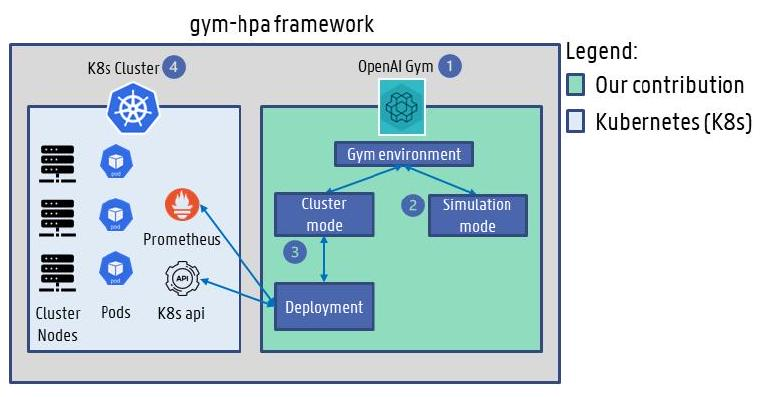
\includegraphics[width=\textwidth]{images/2024_11_17_21ad14b6196e5740bf69g-4.jpg} % Replace with your framework diagram image
    \end{figure}
    \begin{itemize}
        \item Built on OpenAI Gym for training and testing RL agents.
        \item Designed to interact with Kubernetes clusters in real-time.
    \end{itemize}
\end{frame}

% Slide 2: Kubernetes Integration
\begin{frame}{System Architecture: Kubernetes Integration}
    \begin{block}{Key Components}
        \begin{itemize}
            \item \textbf{Prometheus}: Collects metrics from the Kubernetes cluster.
            \item \textbf{K8s API}: Facilitates interaction between Gym and the cluster.
        \end{itemize}
    \end{block}
    \begin{figure}
        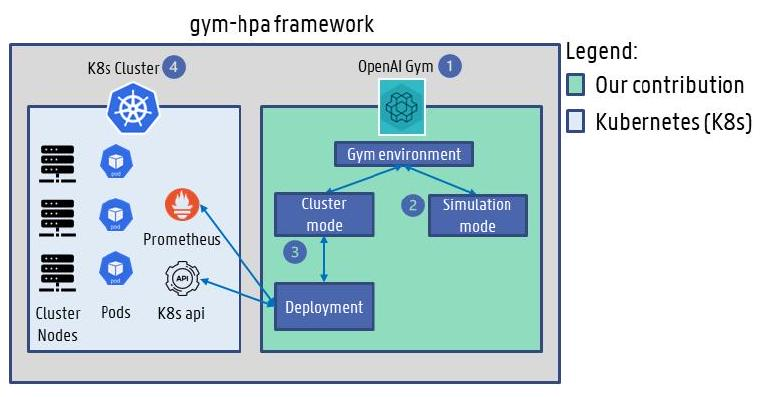
\includegraphics[width=0.8\textwidth]{images/2024_11_17_21ad14b6196e5740bf69g-4.jpg} % Use the image showing Kubernetes interaction
    \end{figure}
    \begin{itemize}
        \item Gym environment receives state data from Kubernetes.
        \item Reinforcement learning agents provide scaling actions.
    \end{itemize}
\end{frame}

% Slide 3: Modes of Operation
\begin{frame}{System Architecture: Modes of Operation}
    \begin{block}{Two Operational Modes}
        \begin{itemize}
            \item \textbf{Cluster Mode}: Real-world deployments with live K8s clusters.
            \item \textbf{Simulation Mode}: Simulated K8s environment for testing.
        \end{itemize}
    \end{block}

    \begin{figure}
        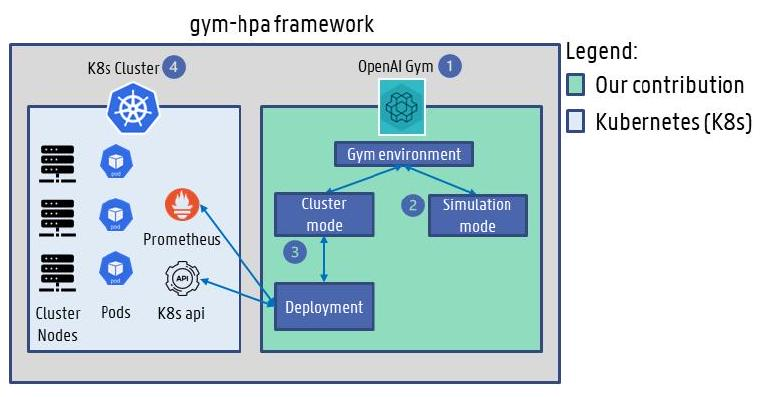
\includegraphics[width=0.8\textwidth]{images/2024_11_17_21ad14b6196e5740bf69g-4.jpg} % Replace with correct file name
    \end{figure}

    \begin{itemize}
        \item Safe testing and policy optimization before real deployment.
    \end{itemize}
\end{frame}




% Slide 1: Challenges in Microservice Scaling
\begin{frame}{Challenges in Microservice Scaling}
    \begin{block}{Key Challenges}
        \begin{itemize}
            \item \textbf{Dynamic Workloads}: High variability in traffic patterns.
            \item \textbf{Complex Dependencies}: Microservices have intricate interdependencies $\rightarrow$ possible bottlenecks
            \item \textbf{Resource Allocation Trade-offs}:
            \begin{itemize}
                \item Minimizing cost.
                \item Ensuring low latency.
            \end{itemize}
        \end{itemize}
    \end{block}
\end{frame}

% Slide 2: Case Study - Online Boutique
\begin{frame}{Case Study: Online Boutique Application}
    \textbf{Online Boutique} is a microservices-based e-commerce platform used to evaluate scaling policies.
    \begin{itemize}
        \item 11 services interconnected with HTTP and gRPC.
        \item Frontend interacts with multiple backend services (e.g., CartService, CheckoutService).
    \end{itemize}
    \begin{figure}
        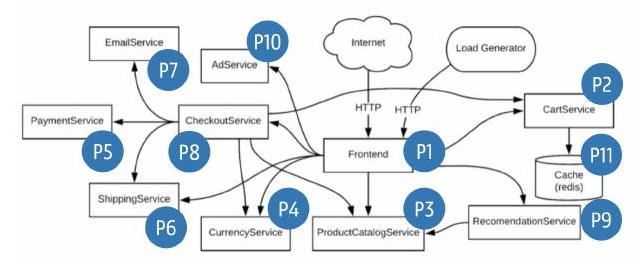
\includegraphics[width=\textwidth]{images/2024_11_17_21ad14b6196e5740bf69g-6.jpg} % Replace with the Online Boutique diagram
        \caption*{Service Dependencies in Online Boutique Application}
    \end{figure}
\end{frame}

% Slide 3: Case Study - Chained Services
\begin{frame}{Case Study: Chained Services Application}
    Mocks interdependent chained services with possible bottlenecks.
    \begin{figure}
        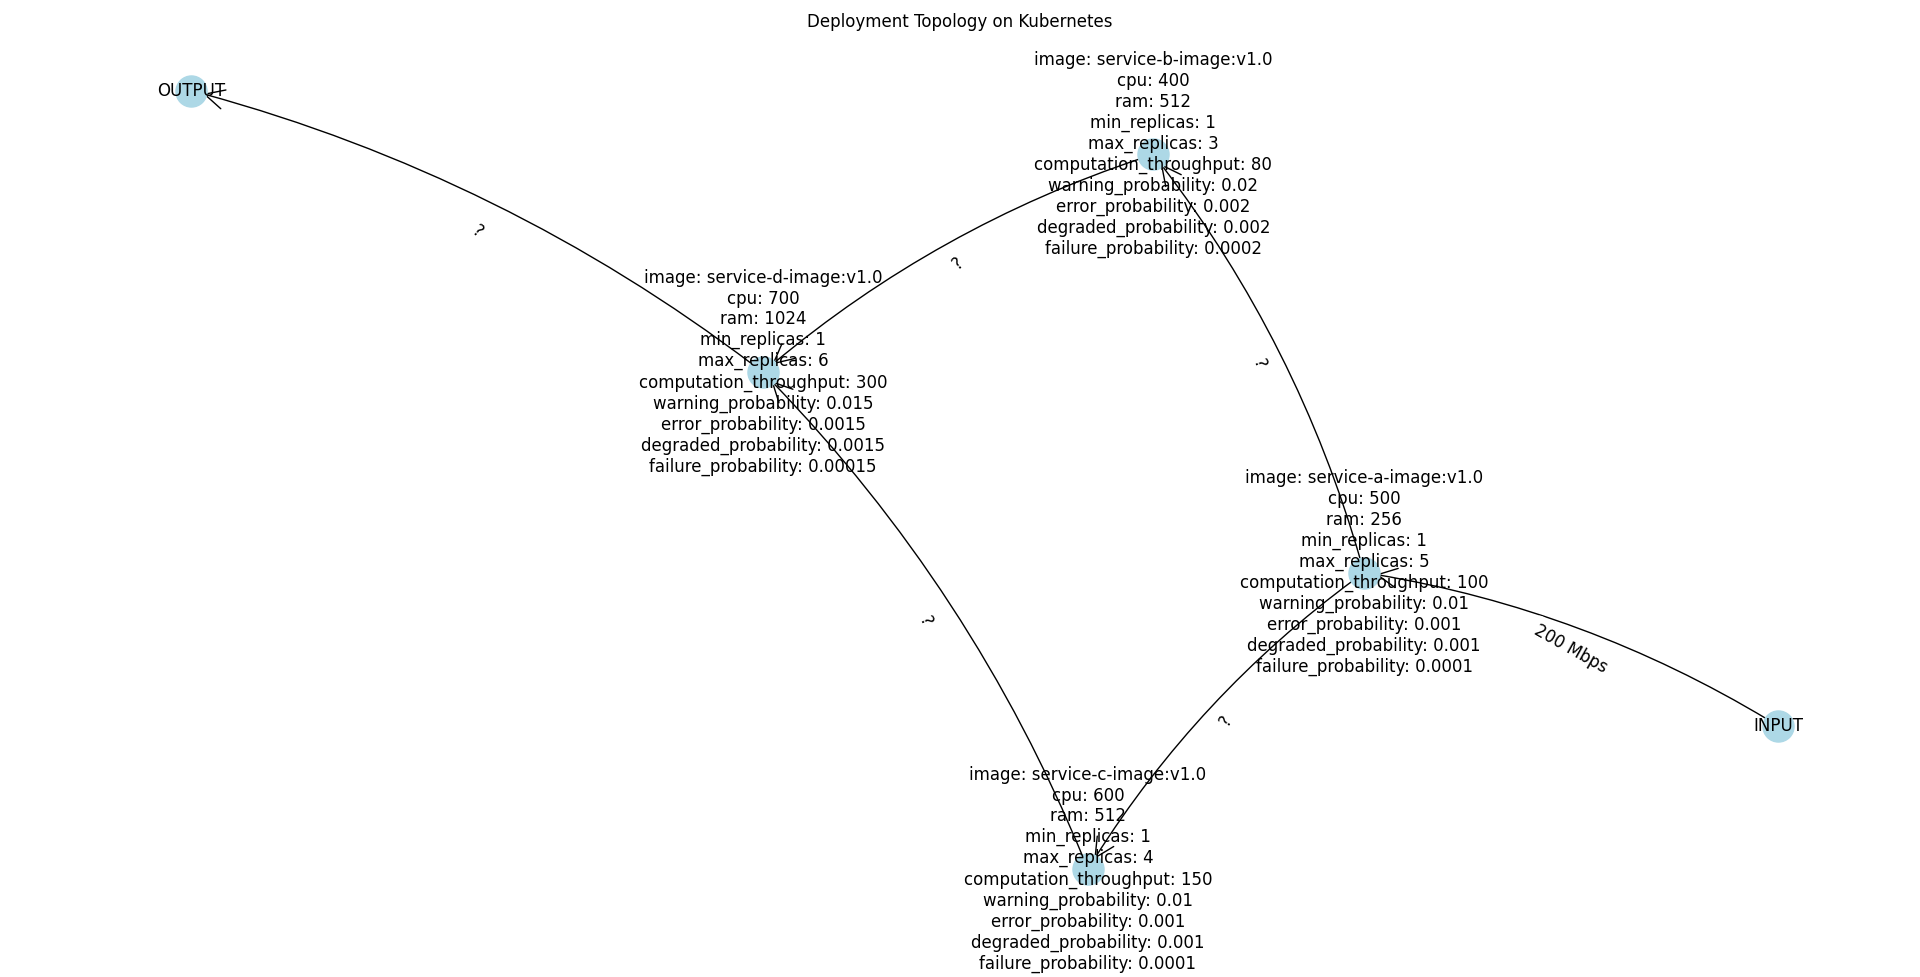
\includegraphics[width=1.1\textwidth]{images/cs_topology.png} % Replace with the Chained Services diagram
        \caption*{Example of the Chained Services Architecture}
    \end{figure}
\end{frame}

% Slide 4: Proposed RL-Based Approach
\begin{frame}{Proposed RL-Based Approach}
    \begin{block}{Reinforcement Learning for Auto-Scaling}
        \begin{itemize}
            \item Define the \textbf{state/observation space}:
            \begin{itemize}
                \item Pod count, CPU usage, latency, etc.
            \end{itemize}
            \item Specify the \textbf{action space}:
            \begin{itemize}
                \item Scale up/down pods dynamically.
            \end{itemize}
            \item Optimize using a \textbf{reward function}:
            \begin{itemize}
                \item Combine cost and latency trade-offs.
            \end{itemize}
        \end{itemize}
    \end{block}

\end{frame}


% Slide 4: Proposed RL-Based Approach
\begin{frame}{Proposed RL-Based Approach}{Observation and Action Space}

    \begin{table}[h]
        \centering
        \caption{Observation Space Structure of k8s-hpa.}
        \resizebox{0.8\textwidth}{!}{ % Réduction automatique pour tenir dans la largeur de la diapositive
        \begin{tabular}{|l|l|}
            \hline
            \textbf{Metric} & \textbf{Description} \\
            \hline
            numPods & Number of deployed pods. \\
            desiredReplicas & Desired number of replicas. \\
            cpuAggr & Total aggregated CPU (in m) of the pods. \\
            memAggr & Total aggregated memory (in Mi) of the pods. \\
            avgTrafficIn & Average received traffic (in Kbps). \\
            avgTrafficOut & Average transmitted traffic (in Kbps). \\
            \hline
        \end{tabular}}
    \end{table}

    \begin{table}[h]
        \centering
        \caption{Action Space Structure of k8s-hpa.}
        \resizebox{\textwidth}{!}{ % Réduction automatique pour tenir dans la largeur de la diapositive
        \begin{tabular}{|c|c|l|}
            \hline
            \textbf{Discrete Set} & \textbf{Action Name} & \textbf{Description} \\
            \hline
            Microservice & D1, D2 & Action triggered on Deployment 1 or 2. \\
            Scaling & DoNothing & No scaling action performed. \\
            & Add-1, Add-2, Add-3 & Add one, two, or three replicas. \\
            & Stop-1, Stop-2, Stop-3 & Remove one, two, or three replicas. \\
            \hline
        \end{tabular}}
    \end{table}

\end{frame}

\begin{frame}{Proposed RL-Based Approach}{Observation and Action Space}

    \begin{itemize}
        \item \textbf{Cost Function:} accurate number of replicas for each microservice deployment, focusing on reducing deployment costs;
        \item \textbf{Latency Function:} latency below a threshold
    \end{itemize}

    \begin{equation}
        \text{getCostReward}(d) =
        \begin{cases} 
            1.0 & \text{if } R_d = \omega_d, \\
            0 & \text{otherwise.}
        \end{cases}
        \label{eq:cost-reward}
    \end{equation}
    
    \begin{equation}
        \text{getLatencyReward}(a) =
        \begin{cases}
            -\Psi_a & \text{if } \Psi_a \leq \tau_a, \\
            -\tau_a & \text{otherwise.}
        \end{cases}
        \label{eq:latency-reward}
    \end{equation}

\end{frame}

% Slide 4: Results - Episode Reward
\begin{frame}{Results: Episode Reward}

    \begin{figure}
        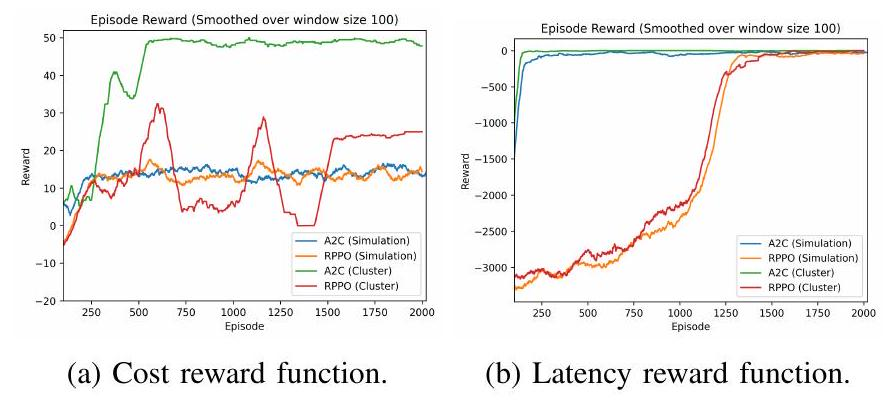
\includegraphics[width=\textwidth]{images/2024_11_17_21ad14b6196e5740bf69g-7.jpg} % Replace with correct file name
        \caption*{Accumulated rewards during training for the Chained Services (CS) application.}
    \end{figure}
    \begin{itemize}
        \item A2C and RPPO algorithms are evaluated in both simulation and cluster modes.
        \item RPPO consistently outperforms A2C in latency optimization.
    \end{itemize}
\end{frame}

% Slide 5: Results - Pods and CPU Usage
\begin{frame}{Results: Number of Pods and CPU Usage}
    \begin{figure}
        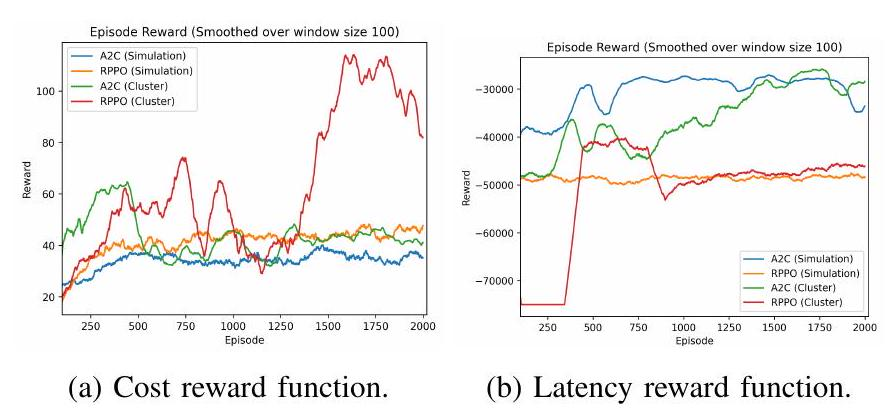
\includegraphics[width=\textwidth]{images/2024_11_17_21ad14b6196e5740bf69g-7(1).jpg} % Replace with correct file name
    \end{figure}
    \begin{itemize}
        \item Deployment efficiency increases with optimized scaling policies.
        \item CPU usage follows expected patterns for scaling algorithms.
    \end{itemize}
\end{frame}

% Slide 5: Results - Pods and CPU Usage
\begin{frame}{Results: Number of Pods and CPU Usage}
    \begin{figure}
        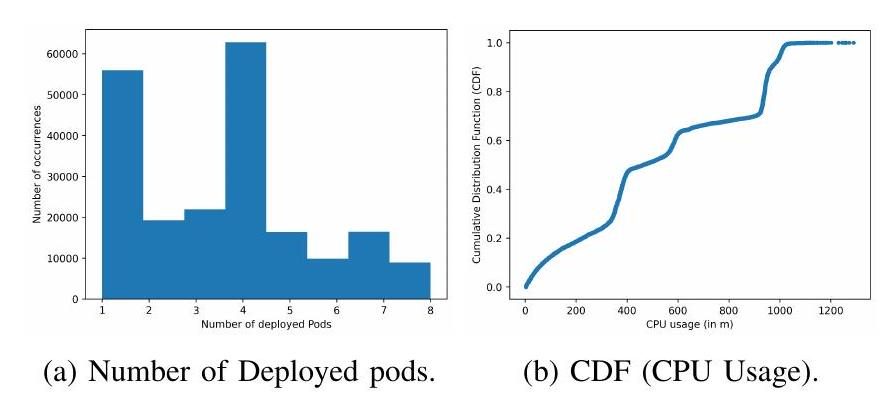
\includegraphics[width=\textwidth]{images/2024_11_17_21ad14b6196e5740bf69g-7(2).jpg} % Replace with correct file name
        \caption*{Accumulated rewards during training for the Online Boutique (OB) application.}
    \end{figure}
    \begin{itemize}
        \item Deployment efficiency increases with optimized scaling policies.
        \item CPU usage follows expected patterns for scaling algorithms.
    \end{itemize}
\end{frame}

% Slide 6: Conclusion
\begin{frame}{Conclusion}
    \begin{itemize}
        \item Proposed a novel K8s-HPA framework for K8s HPA.
        \item Demonstrated effectiveness using A2C and RPPO algorithms.
        \item Future Work:
        \begin{itemize}
            \item Incorporating additional metrics like health, number of warning, errors\dots
            \item Expanding to multi-cluster environments for Multi-Agent Reinforcement Learning.
        \end{itemize}
    \end{itemize}
\end{frame}

% Slide 7: Q&A
\begin{frame}{Questions?}
    \centering
    Thank you for your attention! \\
\end{frame}

\end{document}
